\documentclass[11pt,letterpaper]{article}

\usepackage[margin=1in]{geometry}
\usepackage{graphicx}
\usepackage{amsmath,amssymb}
\usepackage{booktabs}
\usepackage{array}
\usepackage{caption}
\usepackage{float}
\usepackage{xcolor}
\usepackage{url}
\usepackage[hidelinks,bookmarks=true,bookmarksnumbered=true]{hyperref}
\usepackage{siunitx}
\usepackage{titlesec}
\usepackage{setspace}
\usepackage{enumitem}
\usepackage{fancyhdr}

\graphicspath{{figures/}}

% --- typography -------------------------------------------------------
\setlength{\parskip}{6pt}
\setlength{\parindent}{0pt}
\onehalfspacing

\titleformat{\section}
  {\normalfont\Large\bfseries\color{black!85}}{\thesection}{1em}{}
\titleformat{\subsection}
  {\normalfont\large\bfseries\color{black!75}}{\thesubsection}{1em}{}

\pagestyle{fancy}
\fancyhf{}
\fancyhead[L]{\small ECE436 -- IoT Connected SmartHub Dashboard}
\fancyhead[R]{\small \thepage}
\renewcommand{\headrulewidth}{0.4pt}

% --- caption styling --------------------------------------------------
\captionsetup{font=small,labelfont=bf,labelsep=period}

% --- document ---------------------------------------------------------
\begin{document}

% =====================================================================
% TITLE PAGE
% =====================================================================
\begin{titlepage}
    \centering
    \vspace*{2.5cm}

    {\Large\bfseries ROSE--HULMAN INSTITUTE OF TECHNOLOGY\par}
    \vspace{0.8cm}
    {\large DEPARTMENT OF ELECTRICAL AND COMPUTER ENGINEERING\par}
    \vspace{2.5cm}

    {\large Final Report for\par}
    \vspace{0.6cm}
    {\Huge\bfseries IoT Connected SmartHub Dashboard\par}
    \vspace{1.5cm}

    {\large ECE436 -- Internet of Things\par}
    \vspace{2.5cm}

    {\large By\par}
    \vspace{0.6cm}
    {\large Johannes Hirt\par}
    {\large Thiago Costa\par}
    {\large Anar Amartuvshin\par}
    \vspace{2.5cm}

    {\large May 15\textsuperscript{th}, 2026\par}

    \vfill
\end{titlepage}

% =====================================================================
% TABLE OF CONTENTS
% =====================================================================
\pagenumbering{roman}
\tableofcontents
\listoffigures
\listoftables
\clearpage
\pagenumbering{arabic}
\setcounter{page}{1}

% =====================================================================
% EXECUTIVE SUMMARY
% =====================================================================
\section{Executive Summary}
The IoT Connected SmartHub Dashboard is a multi-functional smart desk
system developed using ESP32 microcontrollers in combination with LoRa,
Bluetooth Low Energy (BLE), and Wi-Fi communication
technologies. The system provides
real-time weather updates, music playback, battery status,
environmental sensor data, and nearby BLE devices through an
interactive 7-inch dashboard display.

LoRa communication enables reliable long-distance wireless sensor data
transmission, while BLE supports nearby device scanning and smartwatch
interaction. Wi-Fi is used for web server access, remote interaction,
and Apple Shortcut battery updates.
The project also integrates a camera-based hand-gesture control
system using Edge Impulse machine learning for automatic screen
rotation and user interaction. A 7-inch display is
connected to the main SmartHub device, where all real-time data and
system information are visualized. A heavy-duty servo motor is used
to rotate the display between \ang{0} and \ang{90} orientations for
portrait and landscape viewing modes.

Overall, the SmartHub combines multiple IoT technologies into a single
user-friendly dashboard platform designed to provide students and
everyday users with convenient access to important real-time
information from one centralized desk device.

% =====================================================================
% INTRODUCTION
% =====================================================================
\section{Introduction}
The Internet of Things (IoT) allows devices to connect, communicate,
and share data automatically through the internet and wireless
communication technologies. IoT systems improve convenience,
automation, monitoring, and real-time interaction between smart
devices. This project was developed to provide students with easier
access to multiple smart functions through a single centralized
dashboard system.

The IoT Connected SmartHub Dashboard is a multi-functional smart desk
system developed using two Heltec WiFi LoRa ESP32 development boards
and several additional ESP32-based components.
The system integrates multiple communication technologies including
LoRa for long-distance communication, Bluetooth Low Energy (BLE) for
short-range device interaction, and Wi-Fi for web server access and
remote communication.

The SmartHub supports real-time information such as weather updates,
Spotify music playback, battery status, environmental sensor data, and
nearby BLE device detection. The system also
includes a 7-inch ESP32-based display used to visualize dashboard
information and user interaction. The
display supports both portrait and landscape orientations through a
heavy-duty servo motor system. With the help of
camera-based gesture recognition, users can rotate the screen with
simple hand gestures.

The overall goal of the project is to combine multiple IoT
technologies into a single user-friendly SmartHub device designed for
everyday student use.

% =====================================================================
% REQUIREMENTS / SPECIFICATIONS
% =====================================================================
\section{Requirements and Specifications}

\subsection{Functional Requirements}
\begin{itemize}[leftmargin=*]
    \item The SmartHub shall display real-time weather information.
    \item The system shall display Spotify music playback information.
    \item The system shall display environmental sensor data including
          temperature and humidity.
    \item The SmartHub shall support nearby BLE device scanning and
          detection.
    \item The system shall support long-distance LoRa communication
          between ESP32 nodes.
    \item The SmartHub shall provide Wi-Fi web server access for
          remote interaction and monitoring.
    \item The system shall support camera-based hand gesture
          recognition.
    \item The SmartHub shall support automatic screen rotation using a
          servo motor system.
    \item The dashboard shall support both portrait and landscape
          display orientations.
    \item The system shall support real-time updates for dashboard
          information and sensor values.
\end{itemize}

\subsection{Non-Functional Requirements}
\begin{itemize}[leftmargin=*]
    \item The system shall provide reliable wireless communication
          between subsystems.
    \item The dashboard interface shall remain user-friendly and
          responsive during operation.
    \item The LoRa transmitter node shall support low-power operation
          using deep sleep functionality.
    \item The system shall maintain stable operation during continuous
          runtime.
    \item The project shall support modular subsystem integration for
          easier debugging and maintenance.
    \item The system shall support scalable firmware development using
          PlatformIO environments.
    \item The SmartHub shall support smooth user interaction and
          display rendering using LVGL.
    \item The system shall maintain reliable servo motor operation
          without interrupting communication subsystems.
\end{itemize}

% =====================================================================
% RESEARCH / CURRENT WORK
% =====================================================================
\section{Research and Current Work Review}
The SmartHub Dashboard project started with individual subsystem
testing to ensure that each component operated correctly and fulfilled
its intended purpose. After completing subsystem-level testing, the
project progressed toward full system integration using two Heltec
ESP32 WiFi LoRa development boards and multiple wireless communication
technologies. To complete the physical assembly of the system, a
custom housing structure was implemented to support the main SmartHub
ESP32 board, display stand, and camera holder. After completing the
wiring and hardware integration, the entire system was tested to
verify proper power distribution, subsystem communication, and overall
functionality.

Current development focuses on integrating LoRa communication, BLE
scanning, Wi-Fi web server functionality, environmental sensing,
display rendering, gesture recognition, and power analysis for the
overall SmartHub architecture.

The system currently uses a 7-inch Elecrow ESP32-S3 display running
LVGL and LovyanGFX for the main dashboard
interface. BLE functionality has been
implemented for nearby device scanning and smartwatch communication,
while Wi-Fi supports web server access and Apple Shortcut battery
updates for iPhone and iPad devices. LoRa
communication between ESP32 nodes has been successfully tested using
\SI{915}{\mega\hertz} SX1262 transceivers (TX and RX) for reliable
long-distance environmental sensor data
transmission.

The project also integrates a camera-based hand gesture recognition
subsystem using the Seeed Studio XIAO ESP32S3 Sense module and Edge
Impulse machine learning. The gesture recognition system
currently supports directional gesture detection with approximately
\SI{92.9}{\percent} accuracy.

Additional current work includes subsystem integration, automatic
brightness control, power optimization, battery lifetime estimation,
and final system debugging to improve overall system reliability and
user experience.

% =====================================================================
% DESIGN METHOD AND OVERVIEW
% =====================================================================
\section{Design Method and Overview}
The SmartHub Dashboard was designed using a modular IoT architecture
based on multiple ESP32 microcontrollers and wireless communication
technologies. The system integrates LoRa, Bluetooth
Low Energy (BLE), and Wi-Fi communication into a centralized dashboard
platform for real-time monitoring, interaction, and device
control. The very first
architecture design is shown in Figure~\ref{fig:arch-initial}, while
the final version of the architecture system for the SmartHub is
displayed in Figure~\ref{fig:arch-uml}.

\begin{figure}[H]
    \centering
    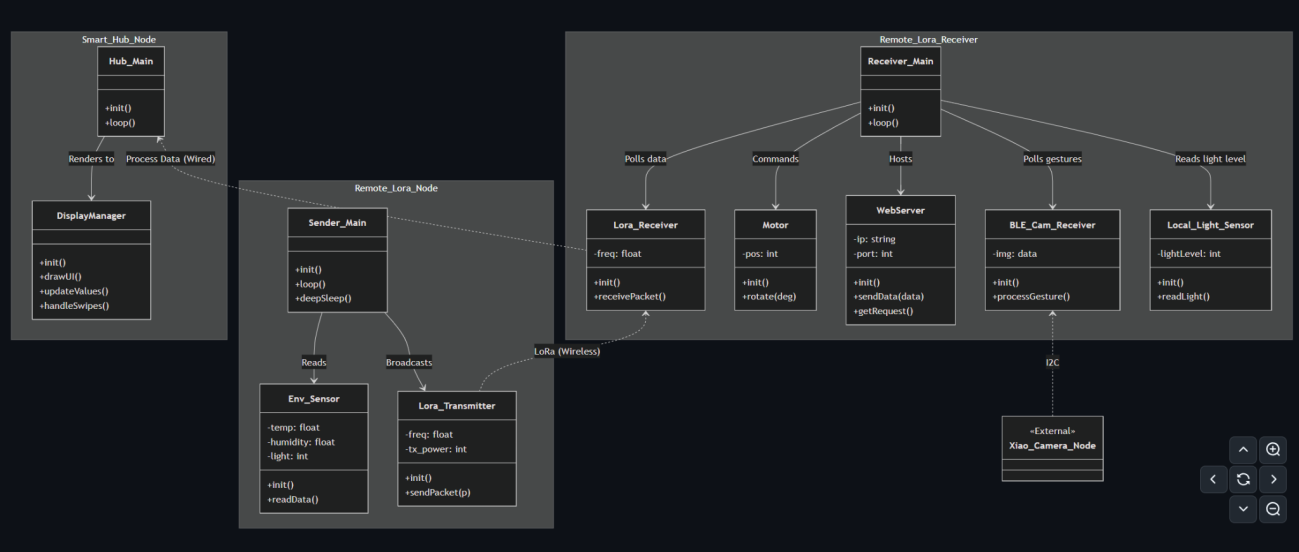
\includegraphics[width=\textwidth]{architecture_uml.png}
    \caption{Overall smartHub Architecture.}
    \label{fig:arch-uml}
\end{figure}

\begin{figure}[H]
    \centering
    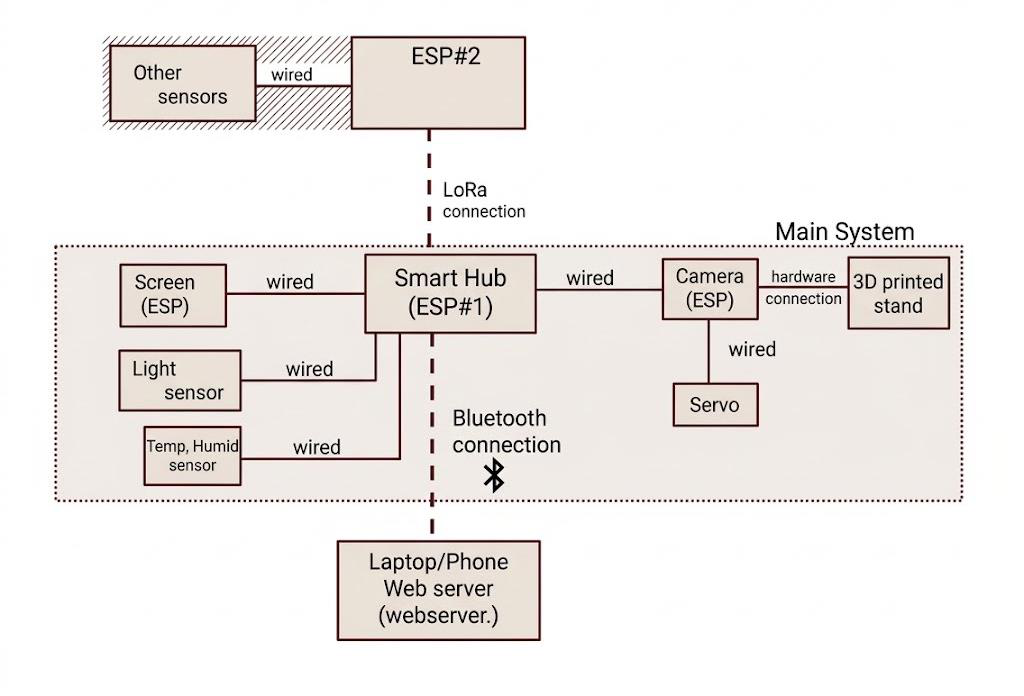
\includegraphics[width=0.7\textwidth]{architecture_initial.png}
    \caption{The first architecture design for the overall system.}
    \label{fig:arch-initial}
\end{figure}

The main SmartHub ESP32 acts as the central controller and connects to
multiple subsystems including the 7-inch Elecrow ESP32-S3 display,
LoRa receiver node, environmental sensors, web server interface,
speaker system, and camera-based gesture recognition
module. The dashboard interface was developed using
LVGL and LovyanGFX to provide a responsive and user-friendly graphical
display system.

LoRa communication is implemented using Heltec ESP32 LoRa development
boards operating at \SI{915}{\mega\hertz} with SX1262 transceivers for
reliable long-distance environmental data
transmission. BLE functionality is used for
nearby device scanning and smartwatch communication, while Wi-Fi
provides web server access, remote interaction, and Apple Shortcut
battery updates.

The system also integrates a camera-based gesture recognition
subsystem using the Seeed Studio XIAO ESP32S3 Sense module and Edge
Impulse machine learning. Gesture detection is used for
automatic screen rotation and dashboard interaction through directional
hand gestures.

The overall design approach focuses on modular subsystem integration,
reliable wireless communication, low-power operation for remote sensor
nodes, and a user-friendly dashboard interface for everyday use.

% =====================================================================
% TEAM CONTRIBUTIONS
% =====================================================================
\section{Team Member Contributions and Work Completed}

\subsection{Anar Amartuvshin}
\begin{itemize}[leftmargin=*]
    \item Integrated BLE and Wi-Fi subsystems into the SmartHub
          dashboard architecture.
    \item Implemented nearby BLE device scanning and RSSI monitoring
          functionality.
    \item Developed Apple Shortcut battery update communication for
          iPhone and iPad devices through Wi-Fi.
    \item Designed and integrated the ``Nearby Devices'' dashboard
          interface.
    \item Assisted with camera dataset collection and gesture labeling
          for machine learning training.
    \item Designed the smartHub closure.
\end{itemize}

\subsection{Johannes Hirt}
\begin{itemize}[leftmargin=*]
    \item Integrated the LoRa receiver subsystem into the SmartHub
          architecture.
    \item Implemented LoRa packet reception, parsing, RSSI monitoring,
          and SNR measurement.
    \item Developed the SmartHub web server and remote-control
          interface.
    \item Integrated environmental sensing and automatic brightness
          control systems.
    \item Performed Packet Delivery Ratio (PDR) testing and received
          power analysis.
    \item Implemented and tested the servo motor subsystem.
    \item Assisted with camera dataset collection and gesture
          labeling.
\end{itemize}

\subsection{Thiago Costa}
\begin{itemize}[leftmargin=*]
    \item Developed the LVGL-based SmartHub dashboard interface for
          the 7-inch display.
    \item Implemented multiple dashboard pages including weather,
          battery, music playback, and BLE device visualization.
    \item Replaced the original OLED implementation with the larger
          touchscreen interface.
    \item Trained and optimized the Edge Impulse hand gesture
          recognition model.
    \item Improved camera gesture recognition performance and machine
          learning integration.
    \item Assisted with overall subsystem integration and UI
          improvements.
\end{itemize}

\subsection{Overall Work Completed}
\begin{itemize}[leftmargin=*]
    \item Full SmartHub dashboard integration using multiple ESP32
          devices.
    \item Successful LoRa communication between ESP32 nodes at
          \SI{915}{\mega\hertz}.
    \item BLE nearby device scanning and smartwatch interaction.
    \item Wi-Fi web server communication and battery update system.
    \item Camera-based hand gesture recognition with approximately
          \SI{92.9}{\percent} accuracy.
    \item Servo motor integration for automatic screen rotation.
    \item Environmental sensing and automatic brightness control.
    \item Power analysis and battery lifetime estimation for multiple
          subsystems.
    \item Real-time dashboard visualization using LVGL and LovyanGFX.
\end{itemize}

% =====================================================================
% VERIFICATION AND RESULTS
% =====================================================================
\section{Verification and Results}
The SmartHub Dashboard subsystems were verified through integration
and communication testing across LoRa, BLE, Wi-Fi, display rendering,
environmental sensing, and gesture recognition systems. Testing
confirmed successful real-time communication between ESP32 nodes and
stable dashboard operation.

LoRa communication testing demonstrated reliable packet transmission
and reception at distances up to \SI{100}{\meter} under free-space
conditions. Packet Delivery Ratio (PDR) measurements
(Figure~\ref{fig:pdr}) showed highly reliable communication
performance, while received power measurements
(Figure~\ref{fig:rxpower}) followed the expected logarithmic path loss
behavior.

\begin{figure}[H]
    \centering
    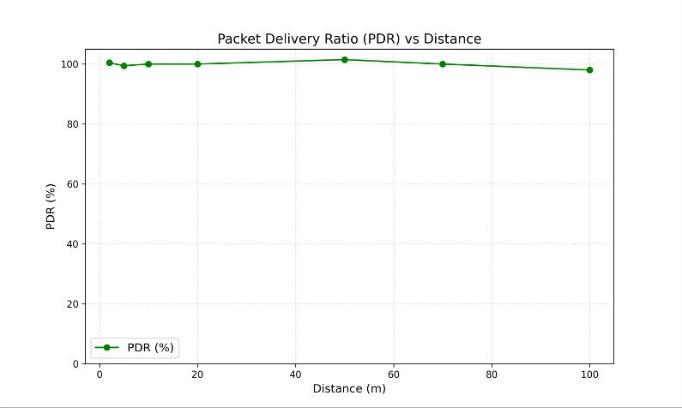
\includegraphics[width=0.75\textwidth]{pdr_plot.png}
    \caption{Packet Delivery Ratio (PDR) vs.\ distance for the
    \SI{915}{\mega\hertz} LoRa link.}
    \label{fig:pdr}
\end{figure}

\begin{figure}[H]
    \centering
    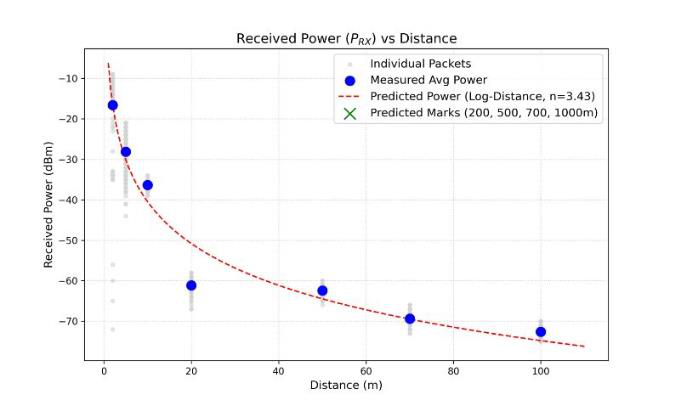
\includegraphics[width=0.75\textwidth]{rx_power_plot.png}
    \caption{Received power vs.\ distance, with a log-distance path
    loss fit \((n = 3.43)\).}
    \label{fig:rxpower}
\end{figure}

BLE testing confirmed successful nearby device scanning, RSSI
monitoring, and smartwatch detection. Wi-Fi testing verified stable
web server communication and successful Apple Shortcut battery updates
for iPhone and iPad devices.

The display subsystem successfully rendered dashboard pages including
weather information, battery status, environmental sensor values, and
nearby BLE devices using the 7-inch ESP32-S3 display. Automatic
brightness adjustment and portrait/landscape display modes were also
successfully tested.

Gesture recognition testing using the ESP32-S3 camera module and Edge
Impulse achieved approximately \SI{92.9}{\percent} accuracy for
directional hand gestures including LEFT, RIGHT, UP, and DOWN.

Power analysis results confirmed stable subsystem operation and
demonstrated the effectiveness of separating the system into multiple
isolated power domains for improved reliability and reduced
power-related communication interruptions.

% =====================================================================
% POWER AND LIFETIME ANALYSIS
% =====================================================================
\section{Power and Lifetime Analysis}
To determine the realistic power requirements and to estimate the
battery lifetime for each subsystem, we performed a measurement-based
power analysis. Current draw was captured for the three independent
power domains in the system: the central SmartHub receiver, the
isolated servo motor, and the remote LoRa transmitter node.

\subsection{Measured Power Sources}
The IoT SmartHub system is partitioned into three power domains, each
with its own supply. Measured current draws are summarized below.

\paragraph{Central SmartHub (Receiver ESP32 \& Display).}
Built from a Heltec WiFi LoRa~32~V3, a 7-inch display, a continuous
Wi-Fi connection, and the web server. Measured current is
\(\sim\SI{470}{\milli\ampere}\) (\SI{0.47}{\ampere}) active
continuous. Powered from wall power via USB-C or a dedicated
\SI{5}{\volt}/\SI{3}{\ampere}+ supply -- driving a 7-inch backlight
and maintaining continuous Wi-Fi/web server connectivity drains too
much current for a battery to be practical.

\paragraph{Actuator (Servo Motor).}
A \SI{20}{\kilogram} RC servo motor. Measured current is a peak of
\SI{8.2}{\ampere}, an average of \SI{2.44}{\ampere}
(\SI{2440}{\milli\ampere}) while active, and \SI{0.06}{\milli\ampere}
at idle. Powered from a separate \SIrange{5}{7}{\volt} battery pack
(e.g., a standard \SI{2000}{\milli\ampere\hour} receiver pack).
Isolating the servo prevents its \SI{8.2}{\ampere} peak spikes from
browning out or resetting the ESP32 microcontroller.

\paragraph{Remote Environment Sensor (Transmitter Node).}
A Heltec WiFi LoRa~32~V3 paired with a DHT11/BHT11 environment sensor.
Measured current is \SI{0.5}{\milli\ampere} during idle/deep sleep
and \SI{129}{\milli\ampere} (\SI{0.129}{\ampere}) while transmitting.
Powered from a \SI{3.7}{\volt} LiPo battery (e.g.,
\SI{2000}{\milli\ampere\hour}) through the Heltec onboard battery
management circuit. This node reads simple sensor data and broadcasts
it via LoRa, so it can leverage deep sleep between readings to
maximize battery life.

\subsection{Transmitter Node Average Current}
To model the power usage of the battery-operated transmitter node, we
divide its operation into two states -- \emph{active} and
\emph{idle/deep sleep} -- and weight each state by the fraction of the
update interval it occupies.

\textbf{Parameters:}
\begin{itemize}[leftmargin=*]
    \item Idle current \(I_{\text{sleep}} = \SI{0.5}{\milli\ampere}\)
    \item Active (transmitting) current
          \(I_{\text{active}} = \SI{129}{\milli\ampere}\)
    \item Active duration \(T_{\text{active}} \approx \SI{2}{\second}\)
    \item Update interval
          \(T_{\text{interval}} = \SI{5}{\minute} = \SI{300}{\second}\)
\end{itemize}

\begin{align*}
I_{\text{avg\_tx}}
&= \frac{I_{\text{active}}\,T_{\text{active}}
        + I_{\text{sleep}}\,(T_{\text{interval}}-T_{\text{active}})}
       {T_{\text{interval}}} \\[4pt]
&= \frac{(\SI{129}{\milli\ampere})(\SI{2}{\second})
        + (\SI{0.5}{\milli\ampere})(\SI{298}{\second})}
       {\SI{300}{\second}} \\[4pt]
&= \frac{258 + 149}{300}\,\si{\milli\ampere}
 = \frac{407}{300}\,\si{\milli\ampere}
 \approx \SI{1.356}{\milli\ampere}.
\end{align*}

\subsection{Receiver Node (SmartHub)}
The central hub remains on continuous wall power due to its constant
high-current requirement. No averaging is needed because the load is
effectively a constant base current:
\[
    I_{\text{base}} = \SI{470}{\milli\ampere}.
\]
Running this load from a \SI{2000}{\milli\ampere\hour} battery would
exhaust the usable capacity in roughly
\(1700/470 \approx \SI{3.6}{\hour}\), which is why the receiver is
permanently wall-powered.

\subsection{Servo Motor Average Current}
The servo is powered by an independent \SIrange{5}{7}{\volt} battery
to isolate its current spikes from the main receiver. Its power usage
is modeled around an hourly sweep, with the idle term retained because
it represents the standing current of the isolated supply rail.

\textbf{Parameters:}
\begin{itemize}[leftmargin=*]
    \item Motor idle current
          \(I_{\text{motor\_idle}} = \SI{0.06}{\milli\ampere}\)
    \item Motor active current
          \(I_{\text{motor\_active}} = \SI{2440}{\milli\ampere}\)
          (average during sweep)
    \item Motor duration \(T_{\text{motor}} \approx \SI{5}{\second}\)
          per sweep
    \item Update interval
          \(T_{\text{interval}} = \SI{1}{\hour} = \SI{3600}{\second}\)
\end{itemize}

\begin{align*}
I_{\text{avg\_servo}}
&= I_{\text{motor\_idle}}
   + \frac{I_{\text{motor\_active}}\,T_{\text{motor}}}
          {T_{\text{interval}}} \\[4pt]
&= \SI{0.06}{\milli\ampere}
   + \frac{(\SI{2440}{\milli\ampere})(\SI{5}{\second})}
          {\SI{3600}{\second}} \\[4pt]
&= \SI{0.06}{\milli\ampere} + \SI{3.39}{\milli\ampere}
 \approx \SI{3.45}{\milli\ampere}.
\end{align*}

\subsection{Battery Lifetime Estimation}
Each battery-powered domain uses a standard
\SI{2000}{\milli\ampere\hour} cell. A safety/efficiency derating
factor of \(0.85\) is applied to account for non-ideal discharge,
self-discharge, and conversion losses, giving a usable capacity of
\[
    C_{\text{usable}} = \SI{2000}{\milli\ampere\hour} \times 0.85
                     = \SI{1700}{\milli\ampere\hour}.
\]

\paragraph{Transmitter Node Lifetime.}
\begin{align*}
t_{\text{tx}}
&= \frac{C_{\text{usable}}}{I_{\text{avg\_tx}}}
 = \frac{\SI{1700}{\milli\ampere\hour}}{\SI{1.356}{\milli\ampere}}
 \approx \SI{1253}{\hour} \\[2pt]
&\approx \SI{52}{\day}\quad(\text{about } 1.7\text{ months}).
\end{align*}

\paragraph{Servo Battery Lifetime.}
\begin{align*}
t_{\text{servo}}
&= \frac{C_{\text{usable}}}{I_{\text{avg\_servo}}}
 = \frac{\SI{1700}{\milli\ampere\hour}}{\SI{3.45}{\milli\ampere}}
 \approx \SI{492.7}{\hour} \\[2pt]
&\approx \SI{20.5}{\day}.
\end{align*}

\paragraph{Receiver Node.}
At \(I_{\text{base}} = \SI{470}{\milli\ampere}\) continuous, the same
derated \SI{1700}{\milli\ampere\hour} cell lasts only
\(1700/470 \approx \SI{3.6}{\hour}\), so the receiver remains wall
powered.

\subsection{Summary}
Table~\ref{tab:power-summary} consolidates the measured currents,
modeled averages, and estimated lifetimes for the three power
domains.

\begin{table}[H]
    \centering
    \caption{Power and lifetime summary by subsystem.}
    \label{tab:power-summary}
    \small
    \begin{tabular}{@{}l c c c@{}}
        \toprule
        \textbf{Subsystem} & \textbf{Avg.\ current} &
        \textbf{Battery} & \textbf{Lifetime} \\
        \midrule
        Transmitter node (LoRa)
            & \SI{1.356}{\milli\ampere}
            & \SI{2000}{\milli\ampere\hour} LiPo
            & $\sim$\SI{52}{\day} \\
        Servo motor (isolated)
            & \SI{3.45}{\milli\ampere}
            & \SIrange{5}{7}{\volt} pack, \SI{2000}{\milli\ampere\hour}
            & $\sim$\SI{20.5}{\day} \\
        SmartHub receiver
            & \SI{470}{\milli\ampere}
            & Wall power
            & continuous \\
        \bottomrule
    \end{tabular}
\end{table}

The analysis validates the decision to separate the system into three
isolated power domains. Keeping the SmartHub on wall power avoids the
\SI{3.6}{\hour} collapse that a battery-only design would suffer, the
isolated servo supply shields the ESP32 from the motor's
\SI{8.2}{\ampere} startup spikes, and deep-sleep operation on the
remote transmitter allows it to run for roughly \SI{52}{\day} on a
single \SI{2000}{\milli\ampere\hour} LiPo cell.

% =====================================================================
% CONCLUSIONS
% =====================================================================
\section{Conclusions}
The IoT Connected SmartHub Dashboard successfully demonstrates the
integration of multiple IoT technologies into a single user-friendly
smart desk system. The project combines LoRa, Bluetooth Low Energy
(BLE), and Wi-Fi communication with environmental sensing, web server
functionality, graphical dashboard rendering, and camera-based gesture
recognition using ESP32 microcontrollers.

Testing results demonstrated reliable LoRa communication, successful
BLE device scanning, stable Wi-Fi interaction, and accurate hand
gesture recognition performance. Power analysis and battery lifetime
measurements also validated the use of isolated power domains to
improve system stability, communication reliability, and power
efficiency.

Overall, the SmartHub Dashboard provides students and everyday users
with convenient access to useful real-time information through a
centralized and interactive platform while demonstrating the practical
implementation of modern IoT communication, embedded systems, and
edge machine learning technologies.

% =====================================================================
% RECOMMENDATIONS
% =====================================================================
\section{Recommendations}
\begin{itemize}[leftmargin=*]
    \item Improve final subsystem integration and reduce communication
          delays between ESP32 devices.
    \item Continue optimizing the hand gesture recognition model to
          reduce false detections and improve overall accuracy.
    \item Improve power management and battery efficiency for more
          portable system operation.
    \item Add additional environmental sensors to expand monitoring
          capabilities.
    \item Improve the SmartHub user interface with smoother animations
          and improved screen organization.
    \item Expand LoRa communication testing in more realistic indoor
          and outdoor environments.
    \item Implement more secure communication methods for Wi-Fi and
          BLE connections.
    \item Improve hardware organization using a custom 3D-printed
          enclosure and mounting system.
    \item Add cloud connectivity for remote monitoring, synchronization,
          and data storage.
    \item Continue long-term reliability and stress testing under
          continuous system operation.
\end{itemize}


% =====================================================================
% APPENDICES
% =====================================================================
\appendix
\renewcommand{\thesection}{\Alph{section}}
\titleformat{\section}
  {\normalfont\Large\bfseries\color{black!85}}{Appendix \thesection}{1em}{}

\section{System Architecture}
\label{app:sysarch}

\begin{figure}[H]
    \centering
    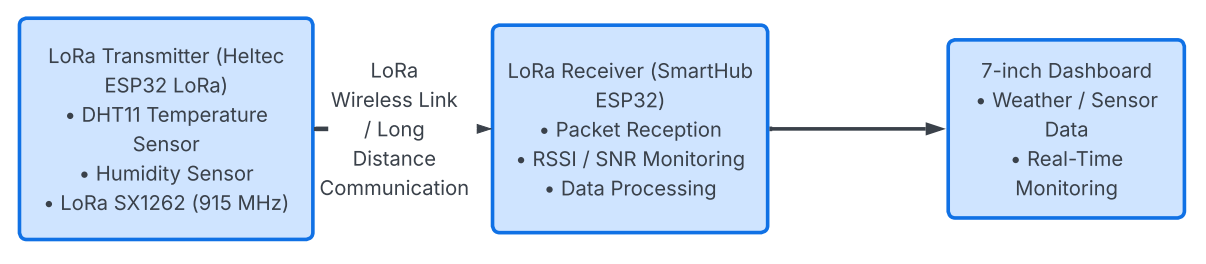
\includegraphics[width=0.85\textwidth]{lora_block.png}
    \caption{LoRa communication block diagram.}
    \label{fig:lora-block}
\end{figure}

\begin{figure}[H]
    \centering
    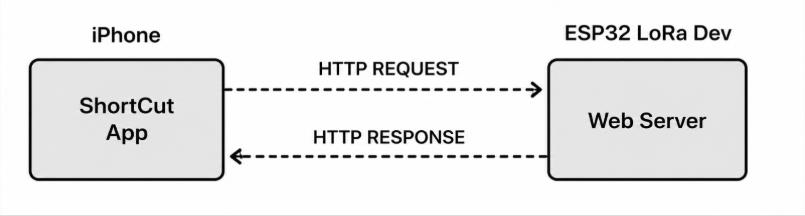
\includegraphics[width=0.7\textwidth]{wifi_ble.png}
    \caption{Wi-Fi and BLE architecture diagram.}
    \label{fig:wifi-ble}
\end{figure}

\begin{figure}[H]
    \centering
    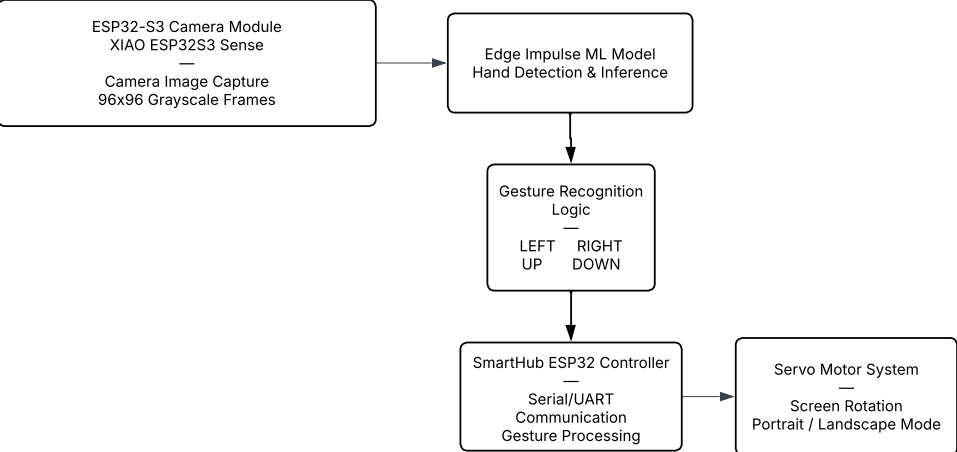
\includegraphics[width=0.7\textwidth]{gesture_arch.png}
    \caption{Camera gesture system architecture.}
    \label{fig:gesture-arch}
\end{figure}

\section{Circuit Diagrams}
\label{app:circuits}

\begin{figure}[H]
    \centering
    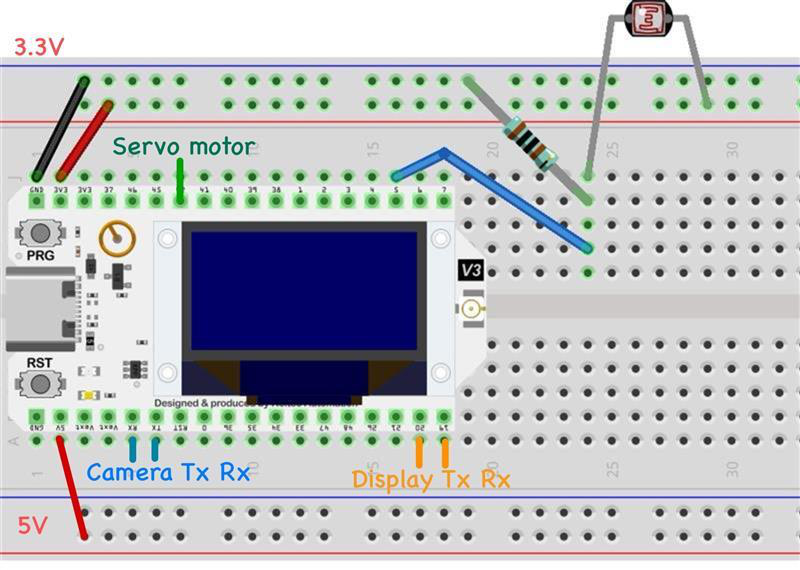
\includegraphics[width=0.65\textwidth]{breadboard.png}
    \caption{Main Hub ESP32 pin connections. Camera and display
    relate to the UART pins.}
    \label{fig:breadboard}
\end{figure}

\section{UI Screenshots}
\label{app:ui}

\begin{figure}[H]
    \centering
    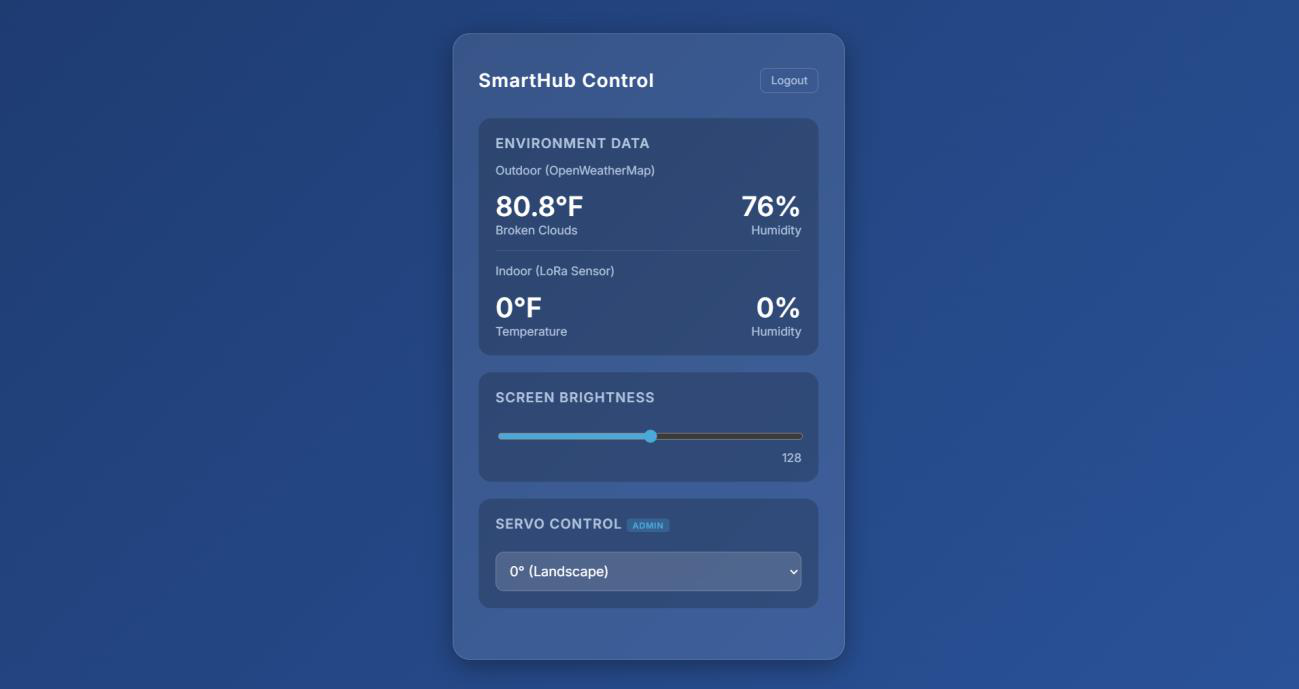
\includegraphics[width=0.55\textwidth]{webserver_ui.png}
    \caption{Web server interface.}
    \label{fig:webui}
\end{figure}

\begin{figure}[H]
    \centering
    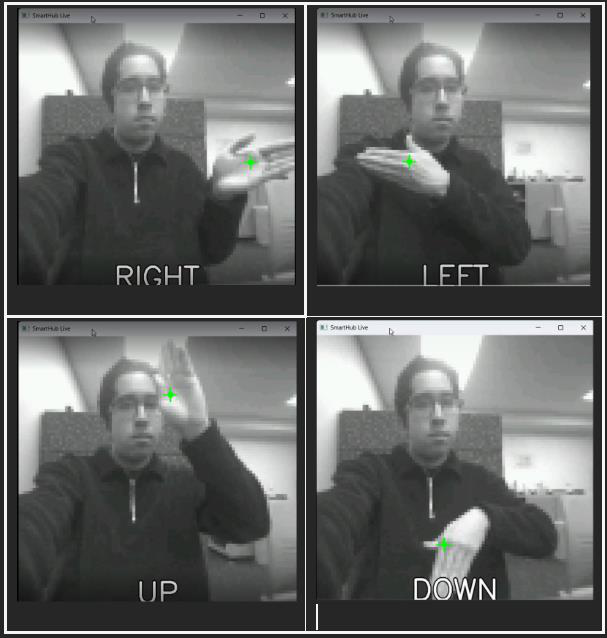
\includegraphics[width=0.55\textwidth]{gesture_demo.png}
    \caption{Gesture recognition demo capturing the four directional
    classes (RIGHT, LEFT, UP, DOWN).}
    \label{fig:gesturedemo}
\end{figure}

\section{Bill of Materials}
\label{app:bom}

\begin{table}[H]
    \centering
    \caption{Bill of Materials}
    \label{tab:bom}
    \begin{tabular}{@{}lll@{}}
        \toprule
        \textbf{Item} & \textbf{Details} & \textbf{Cost (USD)} \\
        \midrule
        Screen              & 7-inch \(800\times480\) ESP32 Screen        & \$53.49 \\
        Camera              & Xiao ESP32-S3 Camera                        & \$21.83 \\
        Motor               & \SI{20}{\kilogram} RC Servo (High Torque)   & \$14.00 \\
        Photoresistor       & In-house (parts room)                       & --      \\
        Humidity sensor     & In-house (parts room)                       & --      \\
        Temperature sensor  & In-house (parts room)                       & --      \\
        \midrule
        \textbf{Total}            &                                        & \textbf{\$89.32} \\
        \textbf{Cost per person}  &                                        & \textbf{\$29.73} \\
        \bottomrule
    \end{tabular}
\end{table}

\end{document}
